\section{Results and Discussion}\label{sec:Results}

% \subsection{Dependence on Number of Fit Points}

% \begin{figure}[p]
%   \centering
%   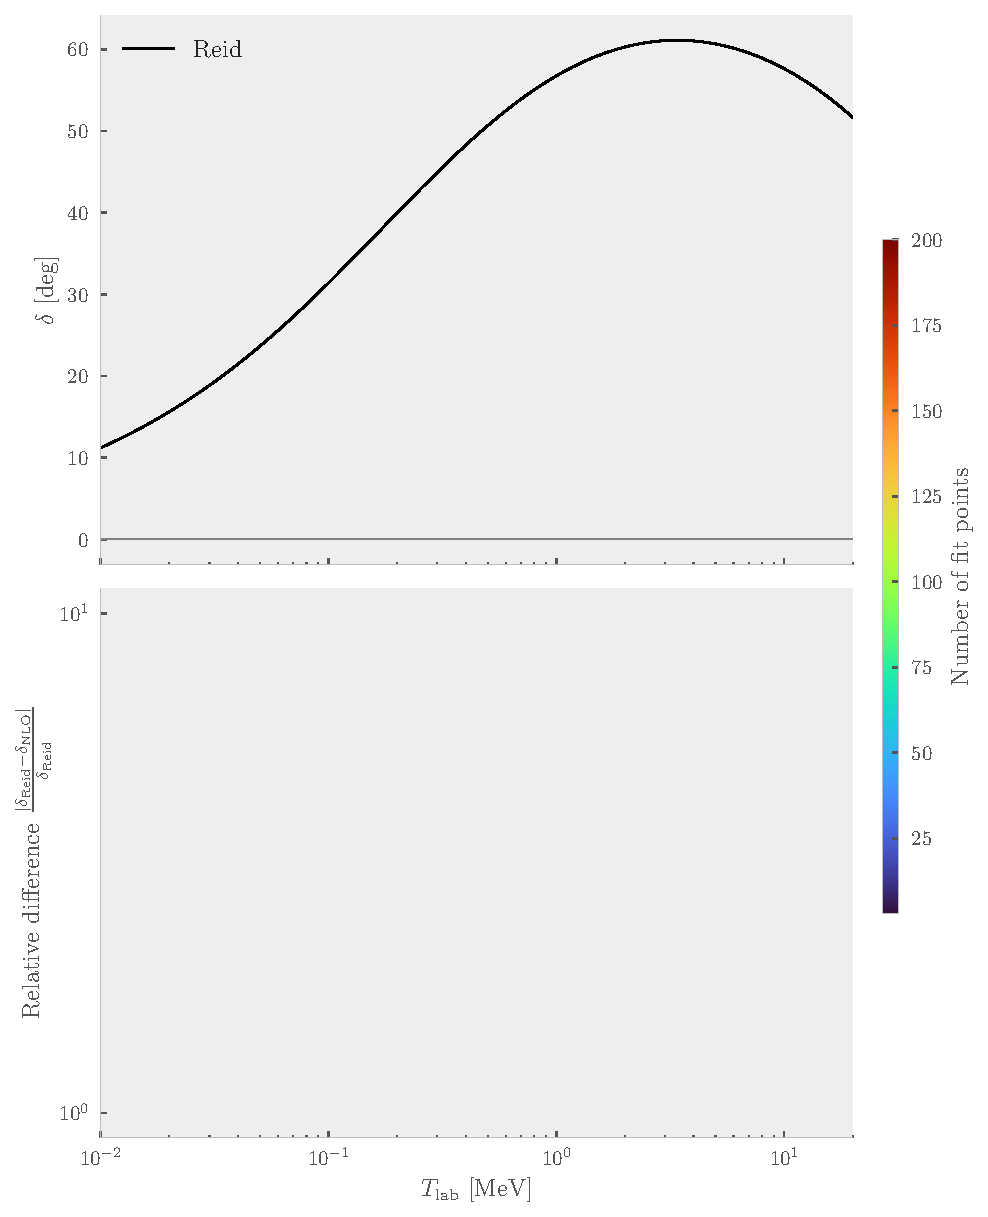
\includegraphics[]{Figures/NLO_points_error.pdf}
%   \caption{\label{fig:points_pointwise} Comparison of Reid and NLO with
%     different number of points used in the minimization. Each curve is fit in
%     the region \([\SI{1e-3}{MeV}, \SI{3}{MeV}]\), resulting in curves shown in the
%     top panel. The pointwise relative error when compared to the Reid potential
%     is shown in the bottom panel. Each curve is colored by the number of points
%     used in the minimization. The minimization gets progressively better as more
%   points are used in the fit.}
% \end{figure}

% \begin{figure}[p]
%   \centering
%   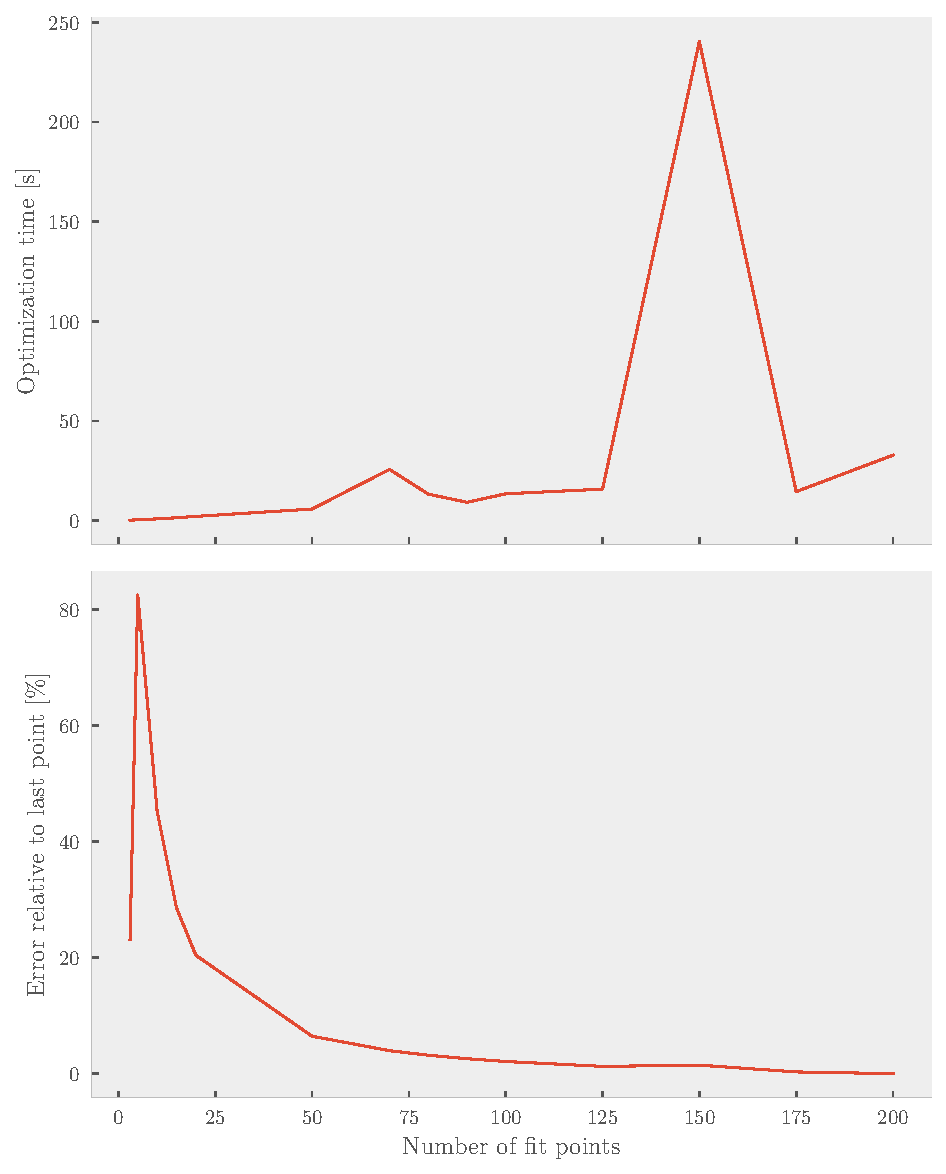
\includegraphics[]{Figures/NLO_dependence_time_error.pdf}
%   \caption{\label{fig:points_time} Illustration of the trade-off between time
%     and accuracy as number of points increases. The time (top panel) increases
%     almost linearly with the number of point, except for the peak \(150\). The
%     error (bottom panel) is calculated as the total relative error when compared
%   to the Reid potential, relative to the last point. Choosing 20 points instead
%   of 200 increases the error by \(20\%\), while \(70\) points yields \(~5\%\)
%   more error.}
% \end{figure}

% \begin{figure}[ht]
%   \centering
%   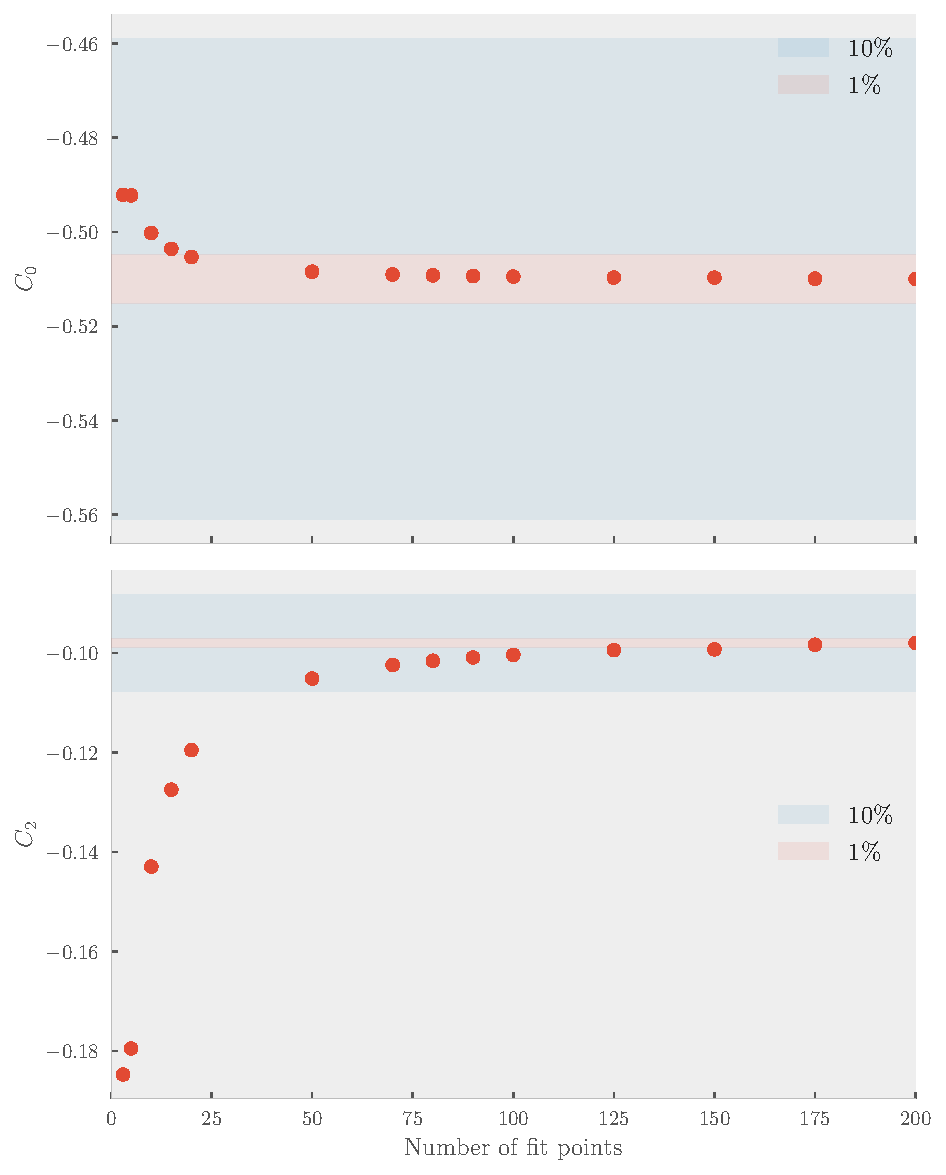
\includegraphics[]{Figures/NLO_coeff_dependence.pdf}
%   \caption{\label{fig:points_coeff} Convergence of the coefficients of NLO as
%   the number of points used in the minimization increases. The shaded bands
%   shows points within \(10\%\) and \(1\%\) of the coefficients value at \(200\)
%   points. At 25 points
%   \(C_{0}\) has already converged to within \(1\%\) of the final value.
%   \(C_{0}\) converges much slower, getting within \(1\%\) of the final value at
%   175 points. }
% \end{figure}

\newcommand{\eend}{E_{\text{end}}}
\subsection{Fit at Low Energies}
The fit is expected to perform best at low energies. What is meant by ``low'' is
arbitrary, usually taken lower than \(1\) MeV. To illustrate why this is ideal,
we perform fits in three different regions, all starting at \mbox{\(10^{-3}\) MeV}
and stopping at \(0.01\), \(1.0\) and \(100\) MeV, respectively. Note that
\(\Lambda=m_{\pi}\), which we will see is suboptimal, but this does not change the
point I will be trying to make. Fifty fit points are used in this section to
exclude too few points as a source of error.

The resulting phase shift and relative error from fitting at low energies are shown in
\cref{fig:lowenergy}. Each order has less
error than the previous in the fit region, and converging to the same error as the
energy increases. However, the improvement from NLO to NNLO is completely
negligible. 

The two NNLO solutions illustrate a common problem with our method
of fitting. A completely unconstrained fit, labeled simply ``NNLO'', give worse
results than a constrained fit, labeled ``NNLO Constrained'', where the
coefficients are forced to be within some hand
picked regions. In general it is very difficult to fit the coefficients of NNLO,
often requiring some bounds in order to keep the solver from getting stuck.

The values and  95\% confidence intervals (CI) of each coefficient is given
in~\cref{tab:lowenergy}. In particular, notice the small bounds on LO and NLO,
indicating that the solver managed to find a stable solution.


\begin{table}[htb]
  \centering
  \begin{tabular}{l|SSSS}
    \multicolumn{5}{c}{Coefficients}\\
    Potential & \(C_{0}\) & \(C_{2}\) & \(C_{4}\) & \(C_{4}^{\prime}\)\\
    \toprule
    LO& -0.53&  &  &  \\
    NLO& -0.54&0.048&  &  \\
    NNLO& -0.50&0.054&-0.99& 0.87\\
    NNLO Constrained & -0.52 & 0.37 & -1.18 & -1.85 \\
    \multicolumn{5}{c}{}\\
    \multicolumn{5}{c}{95\% Confidence Interval}\\
    &\(C_{0}\) & \(C_{2}\) & \(C_{4}\) & \(C_{4}^{\prime}\)\\
    \midrule
    LO &2e-6&  &  &  \\
    NLO& 1e-5& 6e-5&  & \\
    NNLO &3e1& 7e1&6e2&1e3 \\    
    NNLO Constrained &2e1& 4e1 &4e2 & 7e2 \\
  \end{tabular}
  \caption{Coefficients found from fit at \(10^{-3}\) to \(10^{{-1}}\) MeV, as
    well as 95\% confidence intervals of the coefficients. Only the rough
    magnitude is shown for the CI as the numbers change with each execution of
    the fit. [Labels refuse to align. Fix].}
  \label{tab:lowenergy}
\end{table}

\begin{figure}[pt]
  \centering
  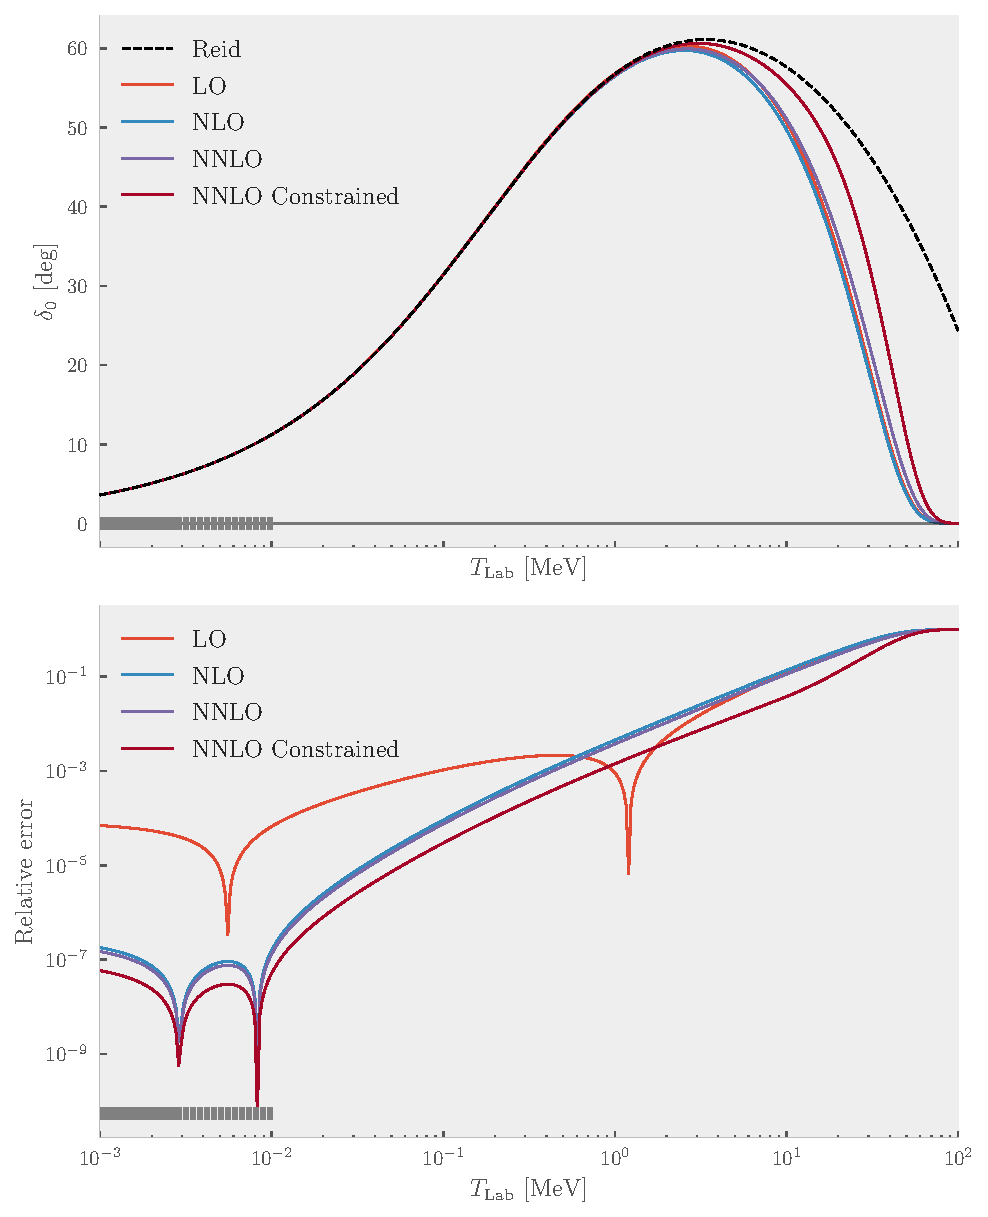
\includegraphics{Figures/lowenergy.pdf}
  \caption{\label{fig:lowenergy} Fit to low energy region with the phase shift
    shown in the top panel and relative error in the lower. The points used in
    the fit is indicated as ticks near the bottom of each plot. LO, NLO and NNLO
  had no limits to their coefficients, while NNLO Constrained was constrained to
 exclude ``unphysical'' phase shifts. The sharp dips are where the curves change
sign.}
\end{figure}

\subsubsection{Fit at Medium Energies}

To see the effect of including higher energies, another fit was performed from \(10^{-3}\)
to \(1\) MeV. The resulting phase shifts and errors are shown
in~\cref{fig:midenergy}. There is a degradation everywhere except around \(1\) MeV
when compared to the low energy fit. In particular, NLO is far worse, being
negligibly better than LO. Another noteworthy change is the increasing number of
dips in the NNLO error, suggesting a more complex shape of the phase shift, as
well as NNLO being better able to fit the Reid potential at energies higher than \(1\) MeV.

The coefficients and CI are shown in~\cref{tab:midenergy}. The degradation in LO
and NLO is reflected in the increased uncertainty of the coefficients by some
orders of magnitude. The CIs of NLO are still small when compared to the value of
the coefficient, indicating that the region used in the fit is worse than the
lower energy. On the other hand, the NNLO has markedly smaller CIs, indicating
that the higher energies are necessary for a good fit.

\begin{table}[htb]
  \centering
  \begin{tabular}{l|SSSS}
    \multicolumn{5}{c}{Coefficients}\\
    Potential & \(C_{0}\) & \(C_{2}\) & \(C_{4}\) & \(C_{4}^{\prime}\)\\
    \toprule
    LO& -0.53&  &  &  \\
    NLO& -0.53&0.015&  &  \\
    NNLO& -0.46&0.44&-2.4& -1.1\\
    \multicolumn{5}{c}{}\\
    \multicolumn{5}{c}{95\% Confidence Interval}\\
              &\(C_{0}\) & \(C_{2}\) & \(C_{4}\) & \(C_{4}^{\prime}\)\\
    \midrule
    LO &1e-5&  &  &  \\
    NLO& 1e-3& 6e-3&  & \\
    NNLO &4e-1& 6e-1&5e0&1e1 \\    
  \end{tabular}
  \caption{Coefficients found from fit at \(10^{-3}\) to \(1\) MeV, as
    well as 95\% confidence intervals of the coefficients. Only the rough
    magnitude is shown for the CI as the numbers change with each execution of
    the fit.}
  \label{tab:midenergy}
\end{table}

\begin{figure}[pt]
  \centering
  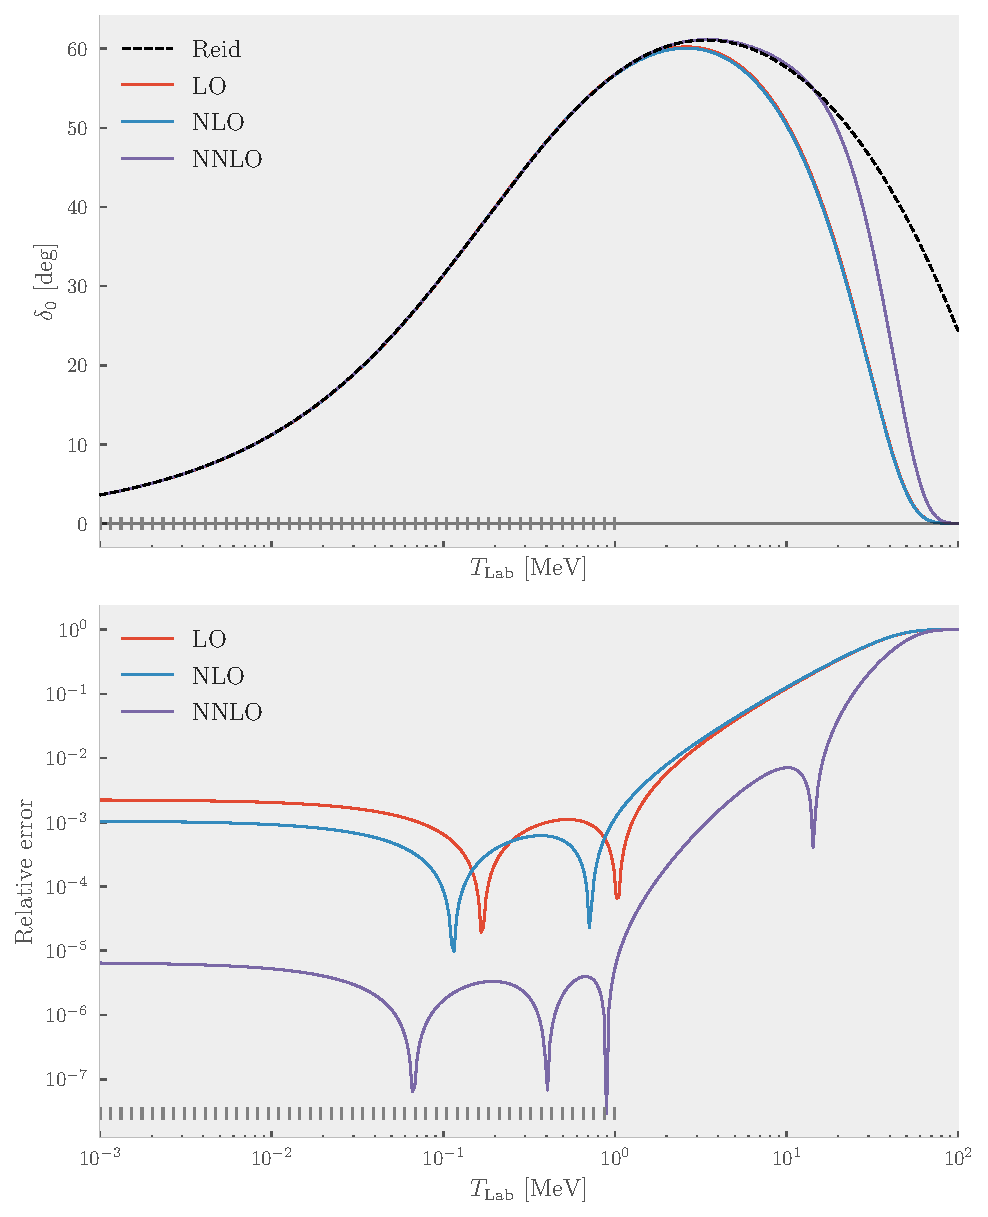
\includegraphics{Figures/midenergy.pdf}
  \caption{\label{fig:midenergy}Fit to the mid energy region with the phase
    shift shown in the top panel and relative error in the lower. The points
    used in the fit are indicated as ticks near the bottom of each plot. No
    constraints were used on the coefficients. When compared to the low energy
    fit, all perform worse in low energy region. NLO does negligibly better than
  LO.}
\end{figure}

\subsubsection{Fit at High Energies}

Yet another fit was performed at energies \(10^{-3}\) to \(100\) MeV, with
results shown in~\cref{fig:highenergy}, and yet again we see an increase in the
relative error. All of the phase shift curves markedly deviate from the phase
shift of the Reid potential. Of the three, NLO has the worst performance, while
the simplest, LO, performs the best.

\cref{tab:highenergy} gives the CIs of the coefficients. The same tale repeats,
with CI becoming increasingly wide. The CIs of the coefficients of NNLO are
utterly useless, spanning six and eight orders of magnitude, illustrating that the
least squares method fails to converge to a good set of coefficients. 

\begin{table}[htb]
  \centering
  \begin{tabular}{l|SSSS}
    \multicolumn{5}{c}{Coefficients}\\
    Potential & \(C_{0}\) & \(C_{2}\) & \(C_{4}\) & \(C_{4}^{\prime}\)\\
    \toprule
    LO& -0.53&  &  &  \\
    NLO& -0.40& -0.58&  &  \\
    NNLO& -0.70&1.3&-3.0& -9.6\\
    \multicolumn{5}{c}{}\\
    \multicolumn{5}{c}{95\% Confidence Interval \((\pm)\)}\\
              &\(C_{0}\) & \(C_{2}\) & \(C_{4}\) & \(C_{4}^{\prime}\)\\
    \midrule
    LO &3e-2&  &  &  \\
    NLO& 1e-1& 6e-1&  & \\
    NNLO &2e6& 3e6&1e8&1e8 \\    
  \end{tabular}
  \caption{Coefficients found from fit at \(10^{-3}\) to \(100\) MeV, as
    well as 95\% confidence intervals of the coefficients. Only the rough
    magnitude is shown for the CI as the numbers change with each execution of
    the fit. [Labels refuse to align. Fix].}
  \label{tab:highenergy}
\end{table}

\begin{figure}[pt]
  \centering
  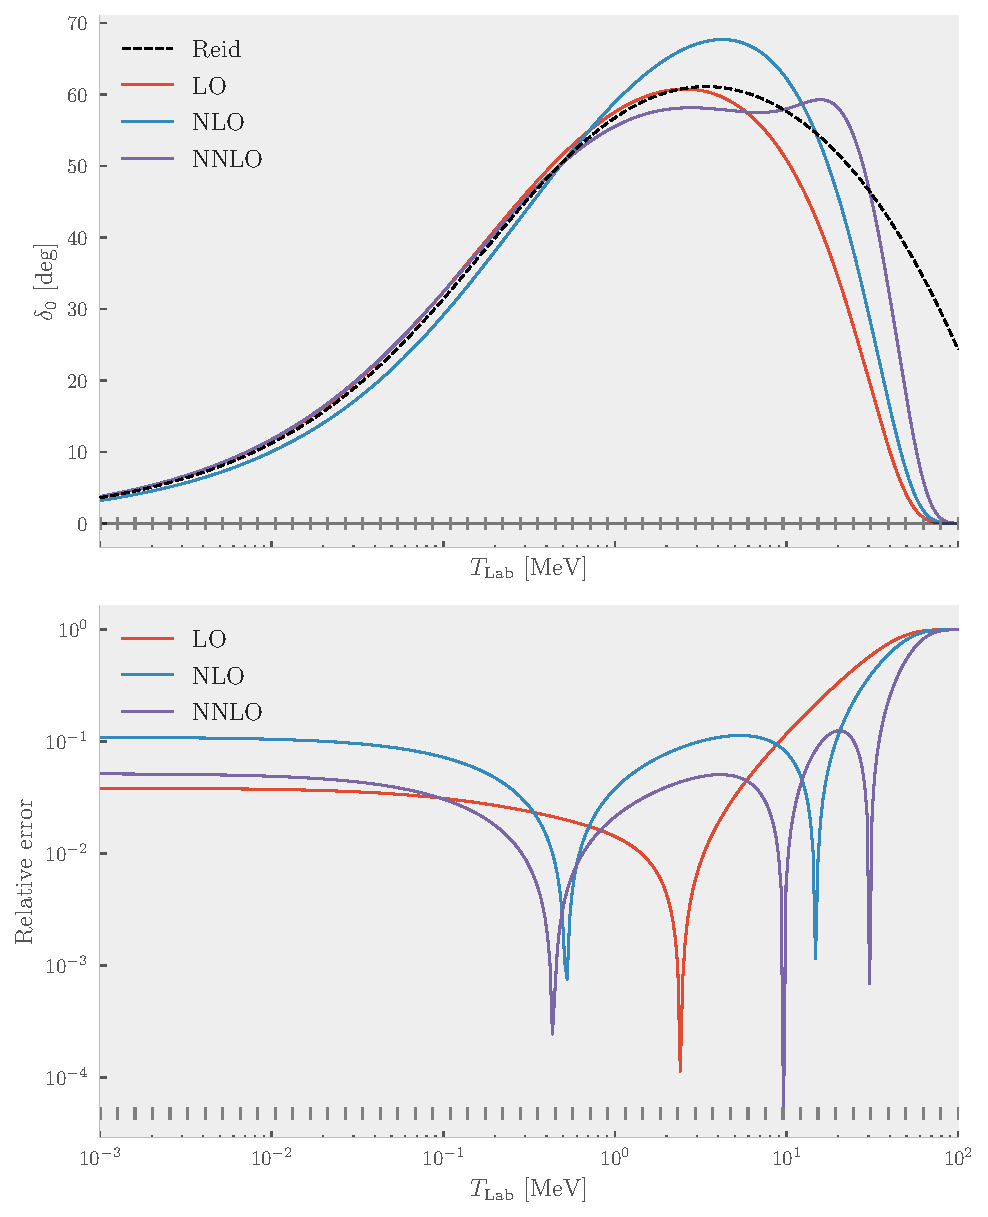
\includegraphics{Figures/highenergy.pdf}
  \caption{\label{fig:highenergy}Fit to the high energy region with the phase
    shift shown in the top panel and relative error in the lower. The points
    used in the fit are indicated as ticks near the bottom of each plot. The
    errors are several order of magnitude greater when compared
    to~\cref{fig:lowenergy} and~\cref{fig:midenergy}}
\end{figure}

\subsubsection{Dependence on Fit Region}

The previous three subsections showed the consequence of fitting LO, NLO and
NNLO to different energies. LO is consistently well
behaved, with fast convergence for the minimization procedures and small
dependence on the hyperparameters. Of course, the reason for this is its
simplicity, with a small parameter space and few parameters that give
nonsensical results. For all of the potentials, the error in the region of fit is lowest for
\(E_{\text{end}} = \SI{1e-2}{MeV}\), but more importantly, the \textit{slope} of
the error is the same. To stress this point, the NLO potential is fitted at a
range of different energies \(\eend{}\) from \num{1e-2} to \SI{100}{MeV},
see~\cref{fig:NLO_region_error}. Two features are obvious. Firstly, a smaller
region of fit will always give a smaller fit error, simply because it is easier
to find arbitrarily good solutions to homogeneous data.  Secondly, the slope
above the fit region remains the same up to about \(5\) MeV. Thus, we will get
fairly similar results if we use regions below \(5\) MeV, in line with the
common rule of thumb of fitting to the most infrared region possible.

The figure also highlights that what we mean by ``error'' depends on the region
of interest. If we are only concerned about low energy physics, then we gain
nothing by fitting at higher energies. If we instead would like an okay
description at a wide range of energies, then perhaps including higher energies
in the fit will yield better results. The black line shows the solution with the
lowest total error in the range \(10^{-3}\) to 100 MeV, suggesting that
using energies up to 10 MeV can be beneficial. In order to be as consistent with
the method of Lepage as possible, energies from \(10^{-3}\) to \(0.1\) MeV is
used from here on.


\begin{figure}[pt]
  \centering
  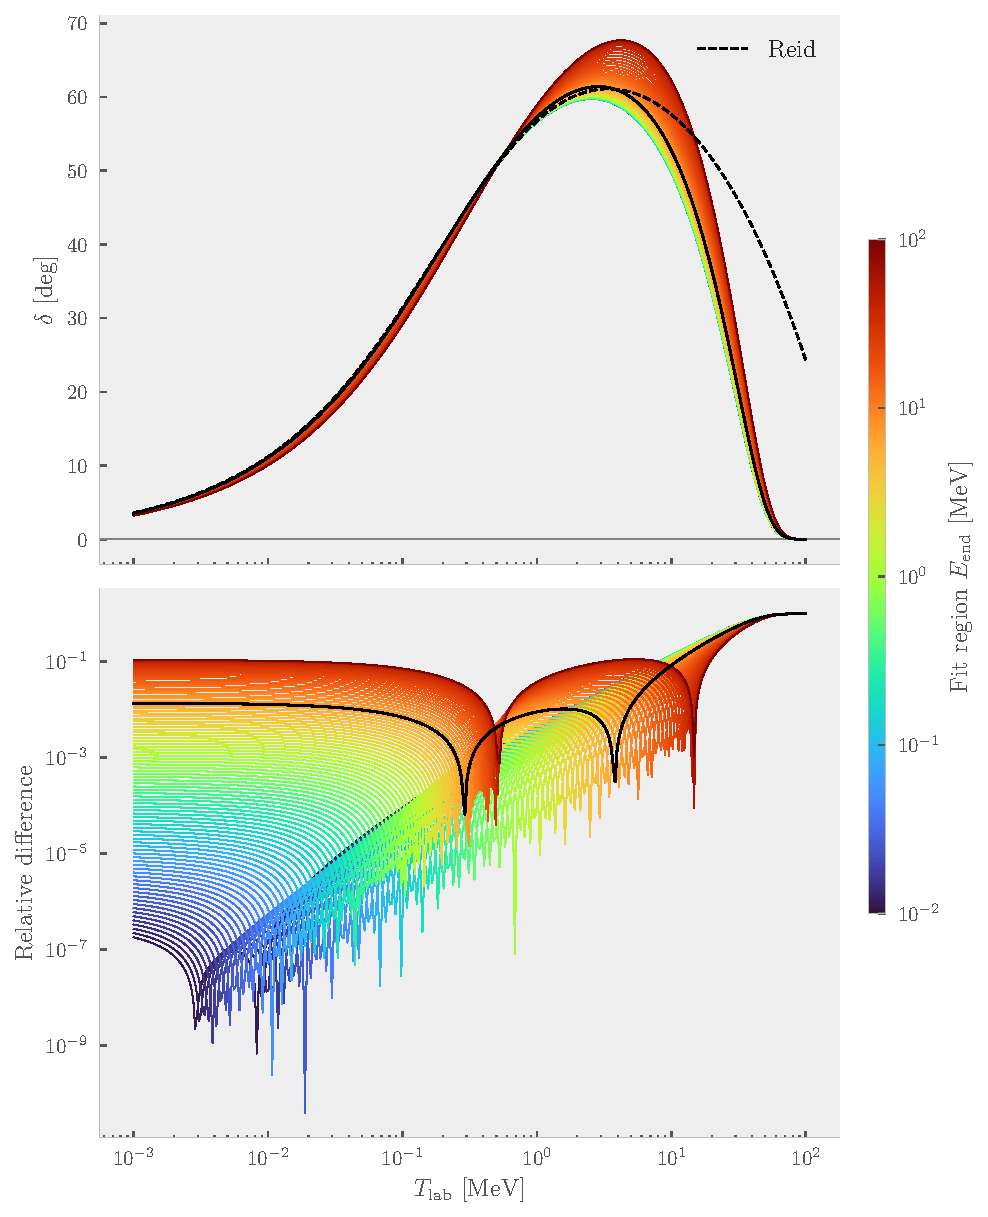
\includegraphics{Figures/NLO_region_error.pdf}
  \caption{\label{fig:NLO_region_error} (Top) The phase shift from NLO and
    (bottom) the relative error. The potential was fit in the region \([10^{-3},
    E_{\mathrm{end}}]\) MeV to illustrate how the fit region affects the result.
    The black line shows the solution with the lowest \textit{total} error in
    the range \(10^{-3}\) to 100 MeV.}
\end{figure}

\FloatBarrier

\subsection{Dependence on \texorpdfstring{\(\Lambda\)}{cutoff}}

For each model the cutoff parameter \(\Lambda\) was varied from \(50\) to
\(600\) MeV, and the models were fitted in the region \([10^{-3},
10^{-1}]\) MeV with 10 points. The results are summarized in
figures~\cref{fig:best_lambdas,fig:lambda_error}. The best values of \(\Lambda\)
are given in~\cref{tab:best_lambdas} and coefficients in~\cref{tab:coefficients}.

The pure \(1\pi\) toy term is a good model when only looking at very low energies.
This is of course expected, as it is precisely the long range interaction that
the pionic terms model. Nor is it surprising that the \(1\pi\) term does not
vary significantly with the value of \(\Lambda\). It does not model any short
range physics, so no higher diagrams are being cut off nor introduced that could
change the value.

The other models show several systematic behaviors. Increasing the order of the
model decreases the error both in the region of fit and above. Adding \(1\pi\)
too decreases the error, as well as systematically increasing the cutoff
\(\Lambda\). LO is particularly nice in this regard, obtaining its minimum right
before \(m_{\pi}\) and failing miserably after, while \(\mathrm{LO}+\pi\) obtains its
minimum above \(m_{\pi}\) and improves the
fit by two orders of magnitude\footnote{Averaged over \num{1e-3} to \SI{100}
  MeV. The improvement is a whopping 4 orders of magnitude in the region of fit.}.

Both LO and NLO break down when
\(\Lambda > m_{\pi}\), but surprisingly NLO carries on its merry way far
beyond. NNLO, on the other hand, fails long before \(\Lambda=m_{\pi}\).  Adding \(1\pi\) improves all models, with NLO\(+\pi\) and
NNLO\(+\pi\) obtaining their minimum at approximately at
\(\Lambda\approx 270\) MeV. That they break down at the same value alludes to
higher energy
physics being involved, perhaps due to the toy nature of our \(1\pi\) term, or
our exclusion of \(2\pi\) and higher order terms. Another possibility is that
perhaps quarks can be resolved near this energy, dooming EFT to become
inaccurate.

Since we are following the approach of Lepage, it is natural to compare our results.
See figures 6 to 8 in~\cite{lepage1997renormalize}. Our methods and data are not
identical, but some general remarks can be made. The slopes in Lepage's errors exhibit the
typical power counting behavior, with each additional order
increasing the log-log slope by approximately \(T_{\mathrm{lab}}^{+2}\). Our
models do not show this. In fact, each order \(\pm 1\pi\) has nearly identical error,
up to a shift.  I do not have any explanation for why this is
the case, except for a failure of the minimization.

However, there is a systematic improvement when adding the \(1\pi\) term.
The term increases the slope of each model by precisely
\(T_{\mathrm{lab}}^{+2}\). This runs counter to Lepage's assertion that
``Evidently one-pion exchange contributes little to the phase shift at most
energies''~\cite[p.~36]{lepage1997renormalize}. I hazard to guess that the
reason for the discrepancy is that the contribution of a term can not be determined
by fitting the term by itself. The different terms capture different physical aspects, so fitting an ``incomplete'' model forces it to account for as many
aspects as possible. In particular, fitting the contact terms by themselves
makes them also fit the long range, low energy data, something they were never
constructed to model. Adding the \(1\pi\) term alleviates this issue, greatly
improving the overall fit. It is perhaps more constructive to compare the
coefficients of the models, as in~\cref{tab:coefficients}. When the \(1\pi\)
term is added, the coefficients of each order more or less align, with each
order term having a lower coefficient\footnote{Both \(C_{4}\) and
  \(C_{4}^{\prime}\) correspond to terms of order $p^{4}$. The fact that they are
  of different sign suggest some cancelation is going on, perhaps due to poor
  fit.}. This constrats to the 
pionless models where the coefficients vary more, and the order of the
coefficients are about the same for each term.  

% When
% fitting the models, I had considerable difficulties with convergence. A
% tell-tale sign of convergence is that the parameters vary smoothly with
% \(\Lambda\). To help
% the algorithm along, I extrapolated the model parameters from where it achieved
% convergence into the region where it had problems, squeezing the bounds as
% \(\Lambda\) increased. This worked well for LO and NLO, but only passably for
% NNLO. 

%There are several reason for
%this. The pionless models are in some sense incomplete, as the derivation of
%their error and dependence on \(\Lambda\) necessitates the inclusion of
%\(1\pi\), and \(2\pi\) for NLO and NNLO. 

\begin{figure}[pt]
  \centering
  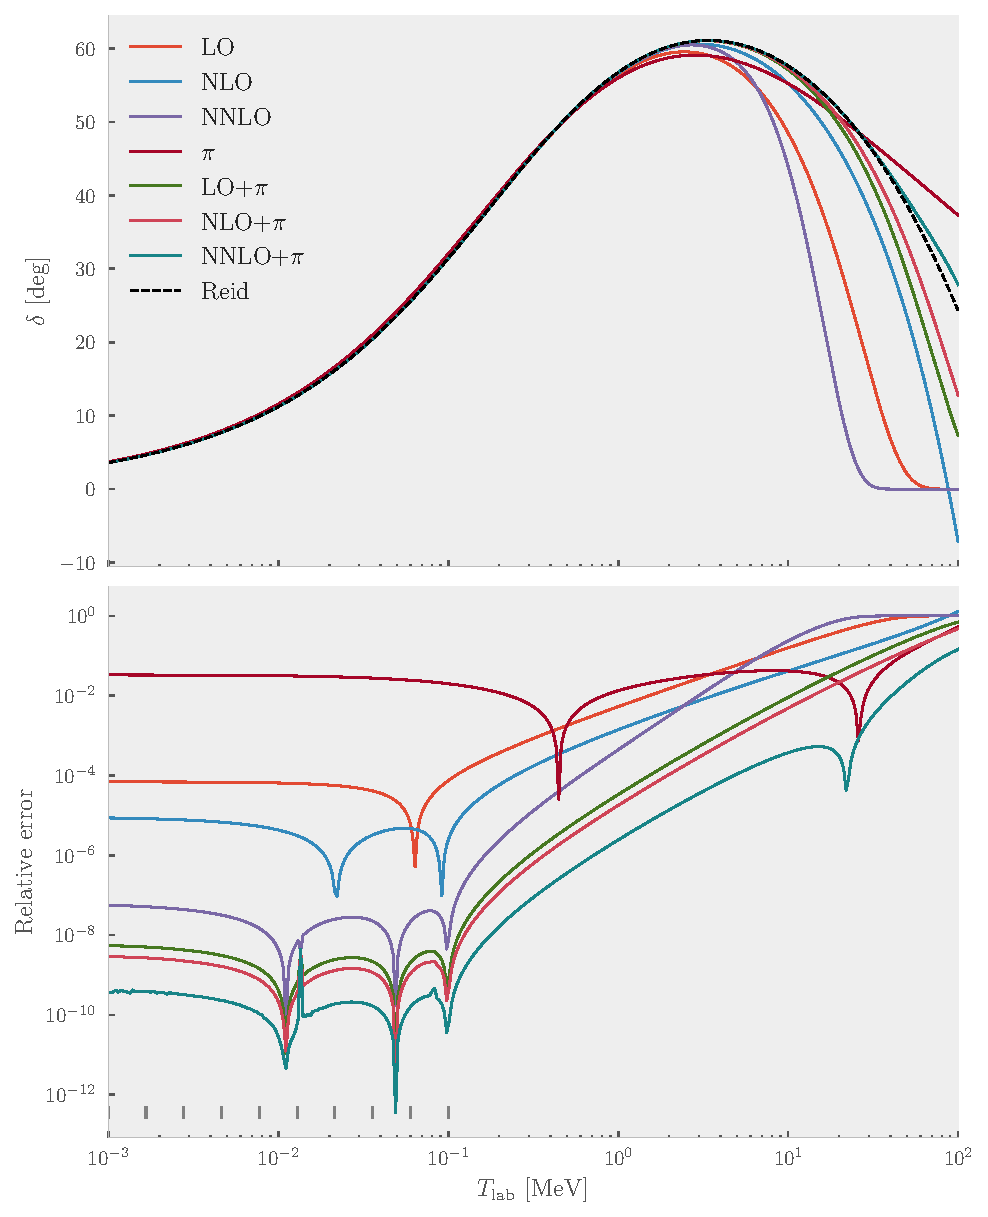
\includegraphics{Figures/best_lambdas_reid.pdf}
  \caption{\label{fig:best_lambdas} (Top) The \(^{1}S_{0}\) phase shift
    calculated from each
    ChEFT potential using their optimal value of \(\Lambda\), along with the
    ``true'' Reid68 potential. \(\pi\) denotes the pure \(1\pi\) toy term. (Bottom) the
    relative error in the aforementioned phase shift. The 10 dashes at the
    bottom mark the points used in the fit. All dips are figments of where the
    absolute value changes sign.}
\end{figure}

\begin{figure}[pt]
  \centering
  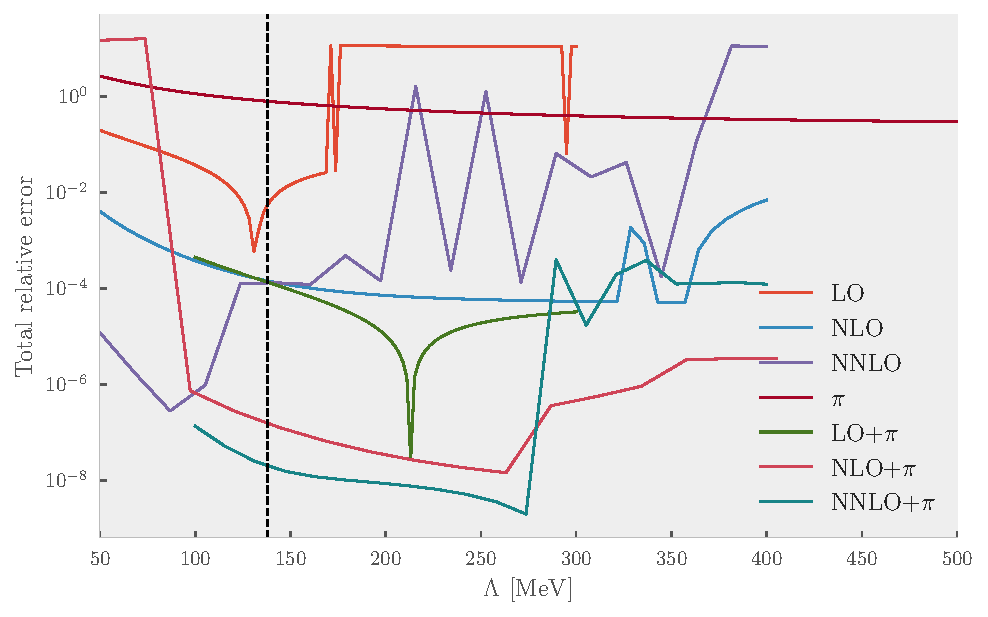
\includegraphics{Figures/lambda_error.pdf}
  \caption{\label{fig:lambda_error} The relative error of the \(^{1}S_{0}\)
    phase shift summed in the region of fit, \num{1e-3} to \num{1e-1} MeV. It is
  plotted against \(\Lambda\) as it runs through \(\approx 50\) to \mbox{\(\approx
  400\) MeV}. \(\Lambda = m_{\pi}\) is shown as a dashed black line. The pionless
potentials with the exception of NLO reach their minima below \(m_{\pi}\), while
the inclusion of the \(1\pi\) toy term raise the minima to about \(270\) MeV.
The pure pion term never achieves a minimum.}
\end{figure}

\begin{table}
  \centering
  \begin{tabular}{l|s}
    Model & \(\Lambda\) [MeV]\\
    \hline
    LO & \num{132}\\
    NLO & \num{357}\\
    NNLO & \num{86}\\
    $\pi$ & \num{>1500}\\
    LO$+\pi$ & \num{213}\\
    NLO$+\pi$ & \num{263}\\
    NNLO$+\pi$ & \num{273}\\
  \end{tabular}
  \caption{The best values of $\Lambda$ for each model. No uncertainties are given
    as no sensible measure could be derived. }
  \label{tab:best_lambdas}
\end{table}

\begin{table}
  \centering
  \begin{tabular}{l|sssss}
    Model & \(C_{0}\) & \(C_{2}\) & \(C_{4}\) & \(C_{4}^{\prime}\) & \(C_{\pi}\)\\\hline
    LO & \num{-5.55e-01} & &&&\\
    NLO & \num{-3.92e-01} & \num{2.48e-01} & &&\\
    NNLO & \num{-6.51e-01} & \num{4.59e-01} & \num{-1.53e+01} & \num{-1.59e+01} &\\
    $\pi$ &&&&& \num{-1.57e-01}\\
    LO$+\pi$ & \num{-2.23e-01} & &&&\num{-7.82e-02} \\
    NLO$+\pi$ & \num{-2.33e-01} & \num{5.43e-02} & &&\num{-6.62e-02} \\
    NNLO$+\pi$ & \num{-2.00e-01} & \num{8.68e-02} & \num{-9.50e-02} & \num{4.53e-02} & \num{-5.67e-02} \\
  \end{tabular}
  \caption{The coefficients of each model. The pionic models have similar
    coefficients, while the non-pionic show more variance. Note also the high
    coefficients for the \(p^{4}\) terms of NNLO, suggesting that the
    minimization failed to find reasonable values. No uncertainties are given as
  no reasonable measure could be found for all of the models, in particular
  NNLO\(\pm \pi\), but for most
  models the minimization converged to several decimal places.}
  \label{tab:coefficients}
\end{table}

\FloatBarrier{}

A possible interjection is that the breakdowns we see are not
due to too high energy physics cropping up, but simply an unfortunate consequence of our fitting
procedure. To justify why this is not the case, we can look at how the parameter
changes as \(\Lambda\) increases. \cref{fig:lambda_NLO} shows the parameters of
NLO\(+\pi\) as \(\Lambda\) changes. All of the parameters converge, yet the
error keeps on increasing beyond \(\Lambda = 263\) MeV. The same convergence is seen
when the bounds on the parameters are removed, although less smooth, hence the bounds
can not be at fault.  Although we may have gotten stuck in local minima, the breakdowns we see
are likely ``true'' breakdowns. By the same reasoning, we can guess that the
minimization of NNLO failed as the parameters show no sign of convergence, while
NNLO\(+\pi\) managed to achieve convergence.


When the minimization was run
several times, all models consistently broke down at around the same values of
\(\Lambda\), giving credence that the optimal values are not flukes. However,
as the number of parameters increase, the minimization gets increasingly
sensitive to initial conditions. For NNLO, another minimum was found for
\(\Lambda = 230\) MeV, but as this solution had three order of magnitude larger
error, it was ignored. Nevertheless, it illustrates the problem of multiple
minima.

\begin{figure}[]
  \centering
  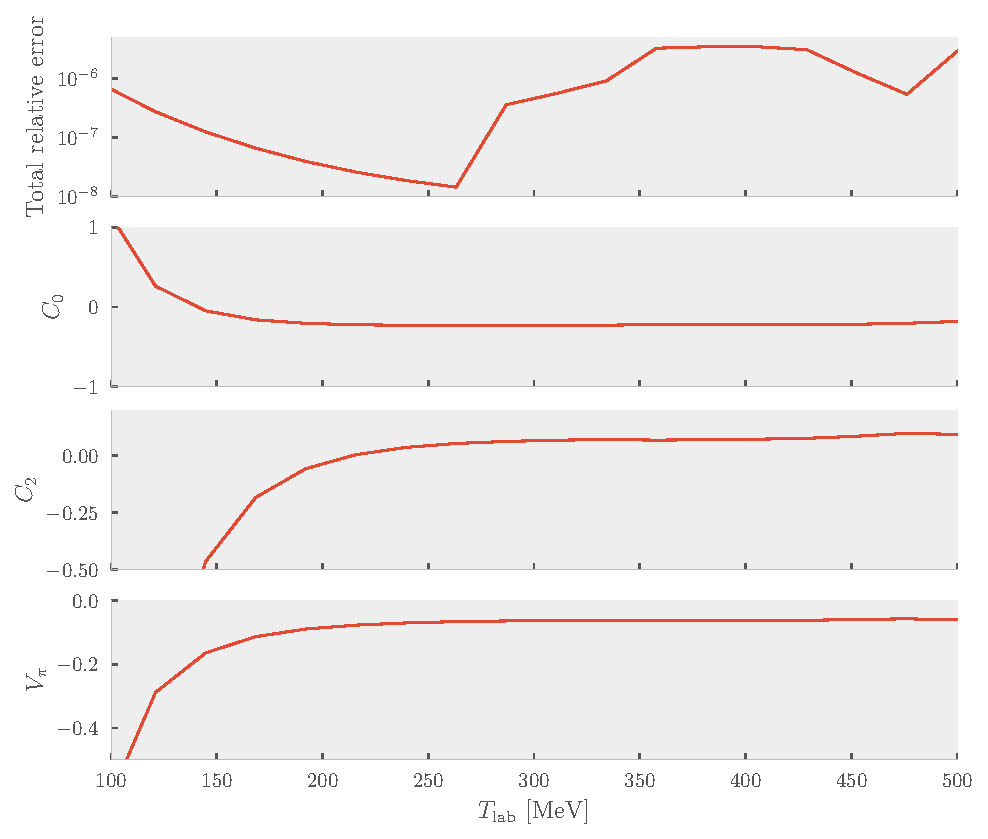
\includegraphics{Figures/lambdas_NLO_coeff.pdf}
  \caption{\label{fig:lambda_NLO} The coefficients of NLO\(+\pi\) and fit error
    as a function of \(\Lambda\). When \(\Lambda > 200\) MeV, the coefficients
    converge while the error keeps decreasing. After the optimal lambda, the
    error quickly increases, even when the coefficients remain near constant.}
\end{figure}

\FloatBarrier{}


\subsection{Search for Power-Law Improvement}

Increasing the chiral order has lead to better models, but the expected power
law improvement has remained missing. I do not know why this is, but suspect it
is mainly due to poor minimization. \cref{fig:best_lambdas} suggests that the
different potentials achieve convergence at different values of \(\Lambda\). In
other words, comparing the results for a specific \(\Lambda\) can lead to a
mediocre  fit for some of the potentials, destroying any power law improvement
that would have been present.

A possible solution is to fit the models for different values of \(\Lambda\) and
find a set of curves that exhibit a power law improvement. The best results are
shown in~\cref{fig:pionless_lambda} and~\cref{fig:pion_lambda}, using values
\(\Lambda=100\) MeV and \(\Lambda=150\) MeV, respectively. The pionless models
exhibit a power-law improvement, with the difference of the exponents being
\(0:0.7:1.6\). The
improvement from NLO to NNLO is the closest to a \(+2\) improvement. The pionic
models has a significantly weaker improvement with \(0:0.98:0.1\). 


\begin{figure}[pt]
  \centering
  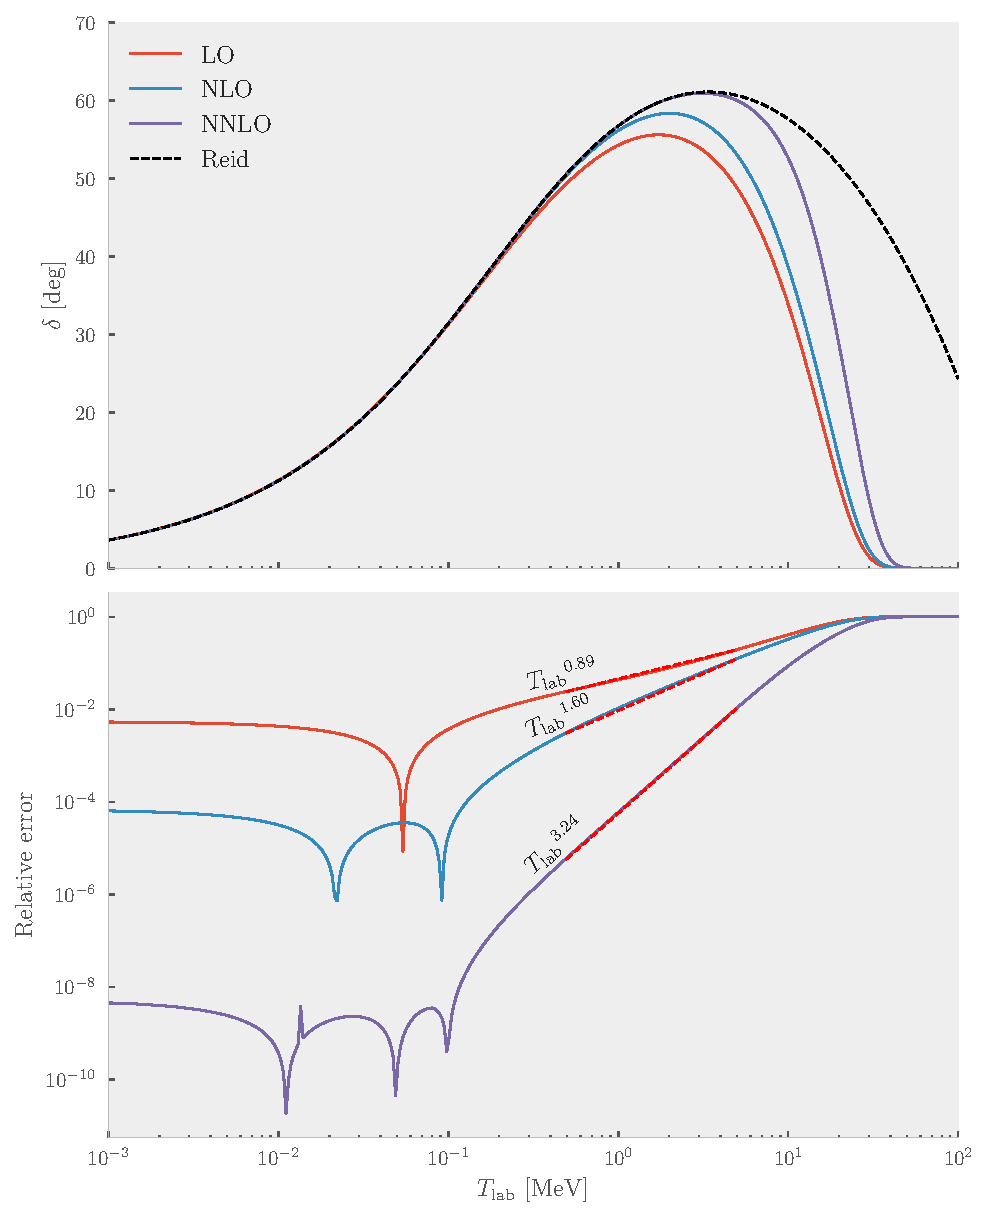
\includegraphics{Figures/pionless_lambda.pdf}
  \caption{\label{fig:pionless_lambda} The phase shift (top) and error in phase
    shift using pionless models. A best fit log-log line is shown from about \(0.5\) to
    10 MeV, along with the exponent. The cutoff was \(100\) MeV.}
\end{figure}


\begin{figure}[pt]
  \centering
  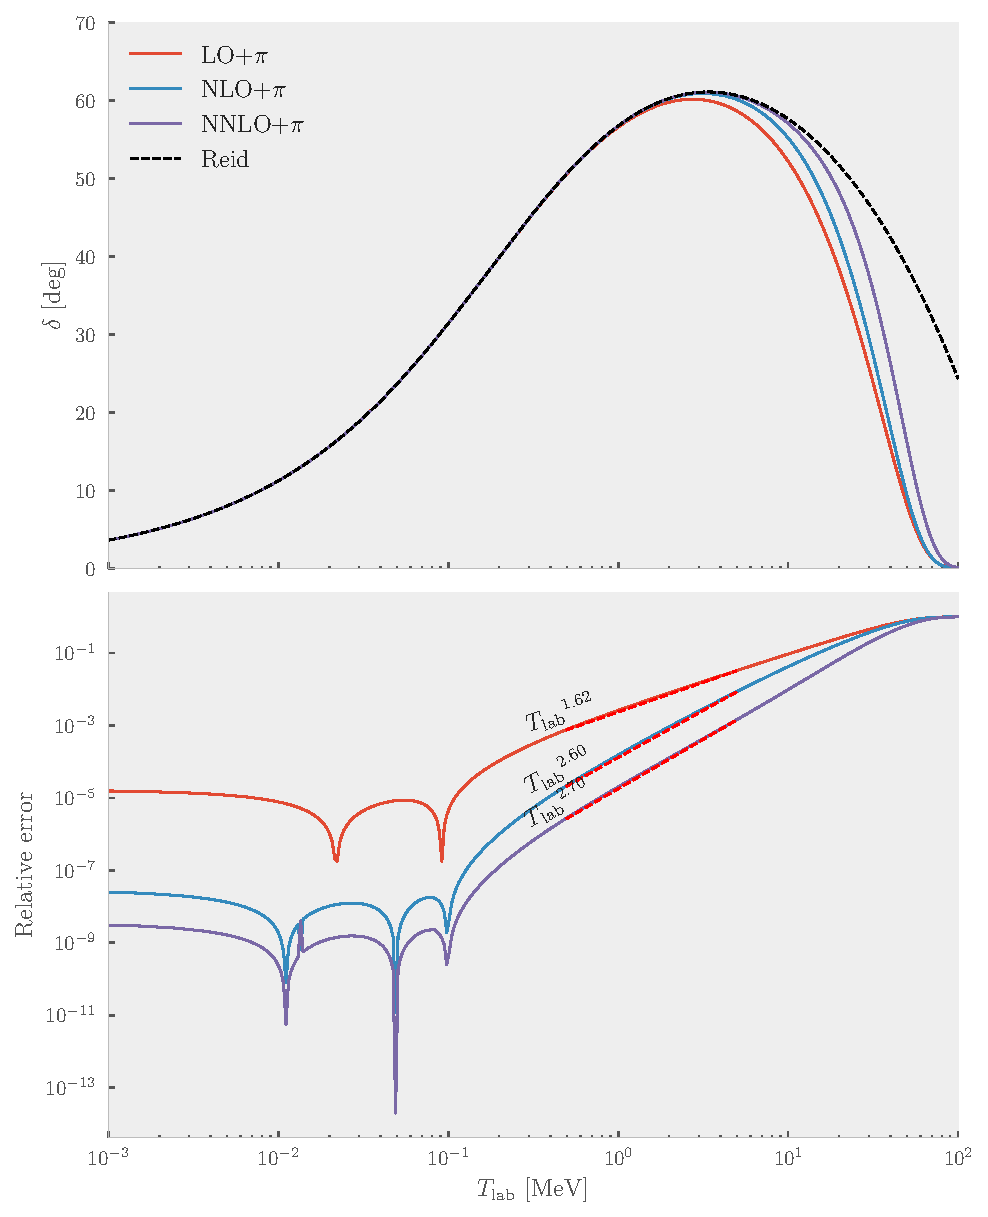
\includegraphics{Figures/pion_lambda.pdf}
  \caption{\label{fig:pion_lambda}  The phase shift (top) and error in phase
    shift using models with \(1\pi\) term. A best fit log-log line is shown from about \(0.5\) to
    10 MeV, along with the exponent. The cutoff was \(150\) MeV.}
\end{figure}


% \subsection{Dependence on cutoff}

% \subsubsection{Pure Pion}

% \begin{figure}[pt]
%   \centering
%   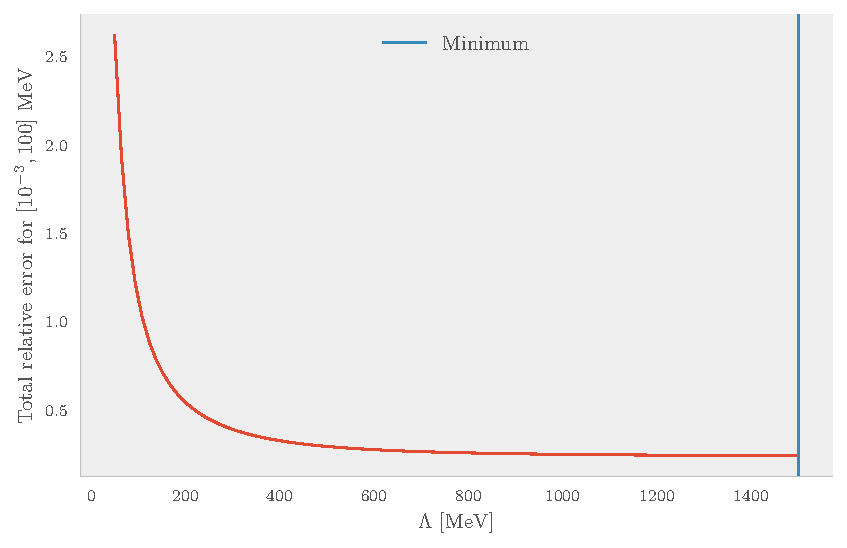
\includegraphics{Figures/lambda_pion_err.pdf}
%   \caption{\label{fig:lambda_pion_err} }
% \end{figure}


% \begin{figure}[pt]
%   \centering
%   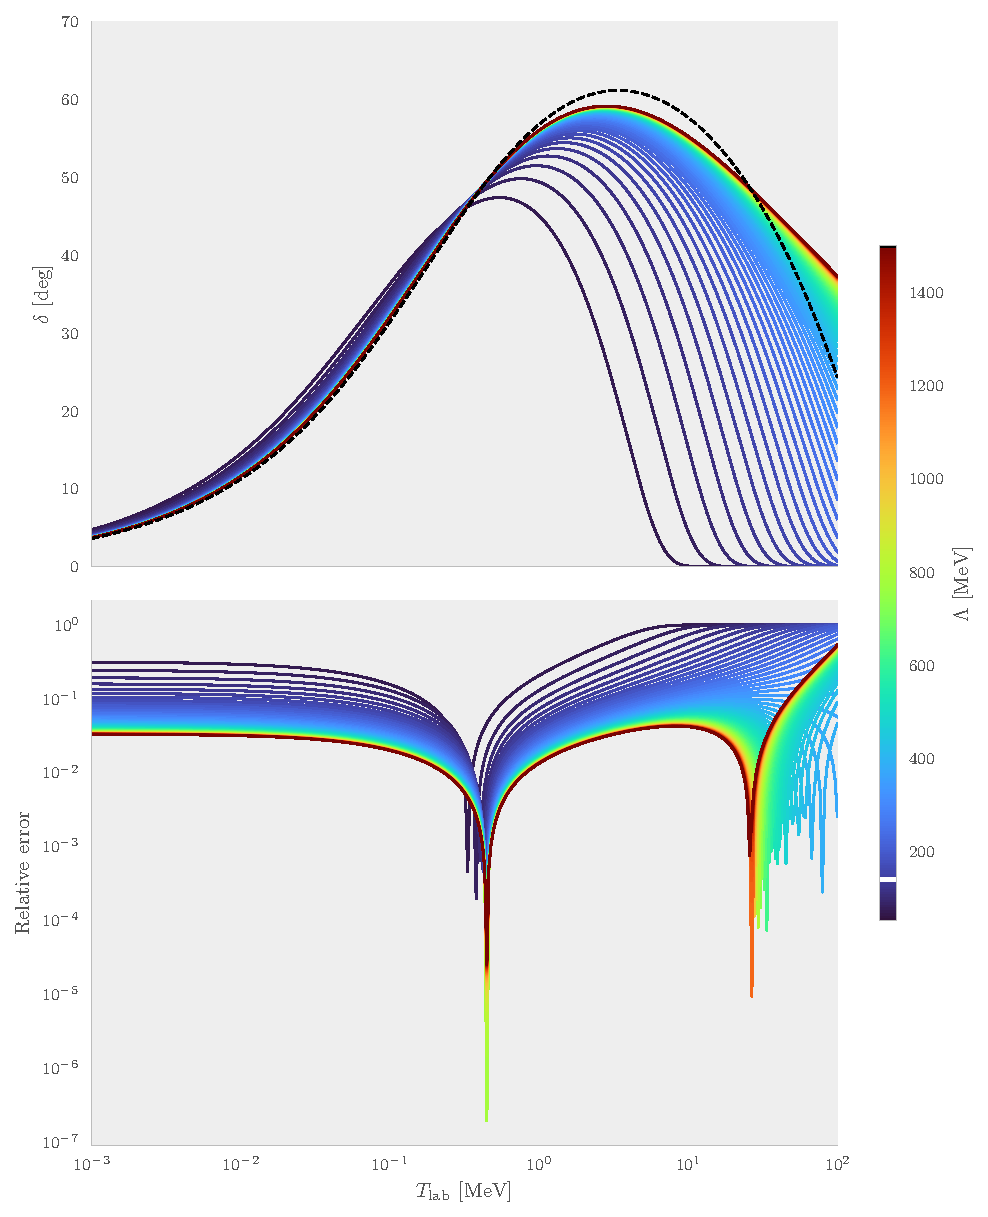
\includegraphics{Figures/lambda_pion.pdf}
%   \caption{\label{fig:lambda_pion} }
% \end{figure}

% \begin{figure}[pt]
%   \centering
%   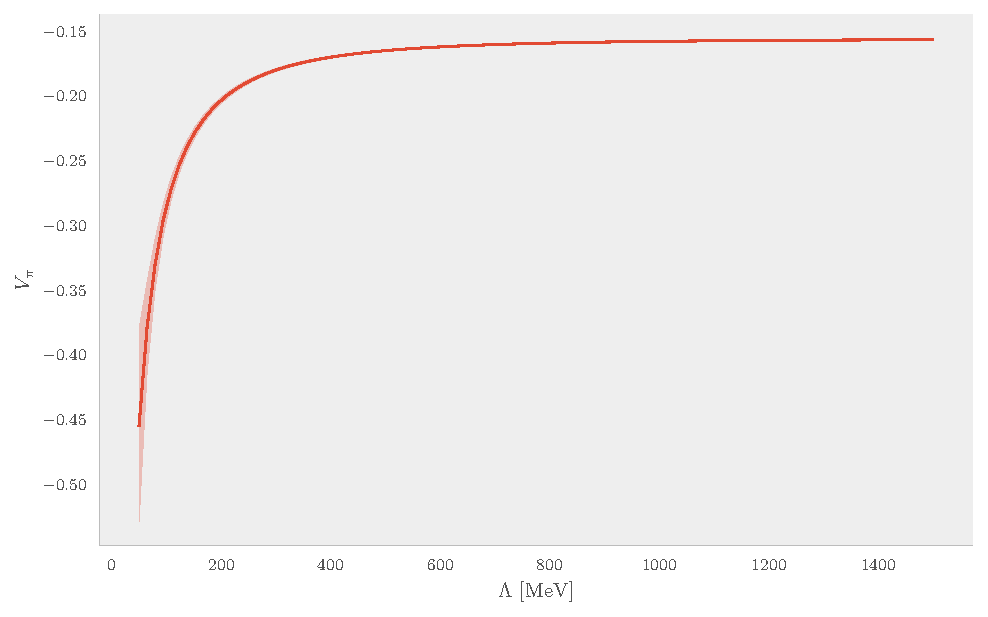
\includegraphics{Figures/lambda_coeff_pion.pdf}
%   \caption{\label{fig:lambda_coeff_pion} }
% \end{figure}

% \subsubsection{LO + Pion}

% \begin{figure}[pt]
%   \centering
%   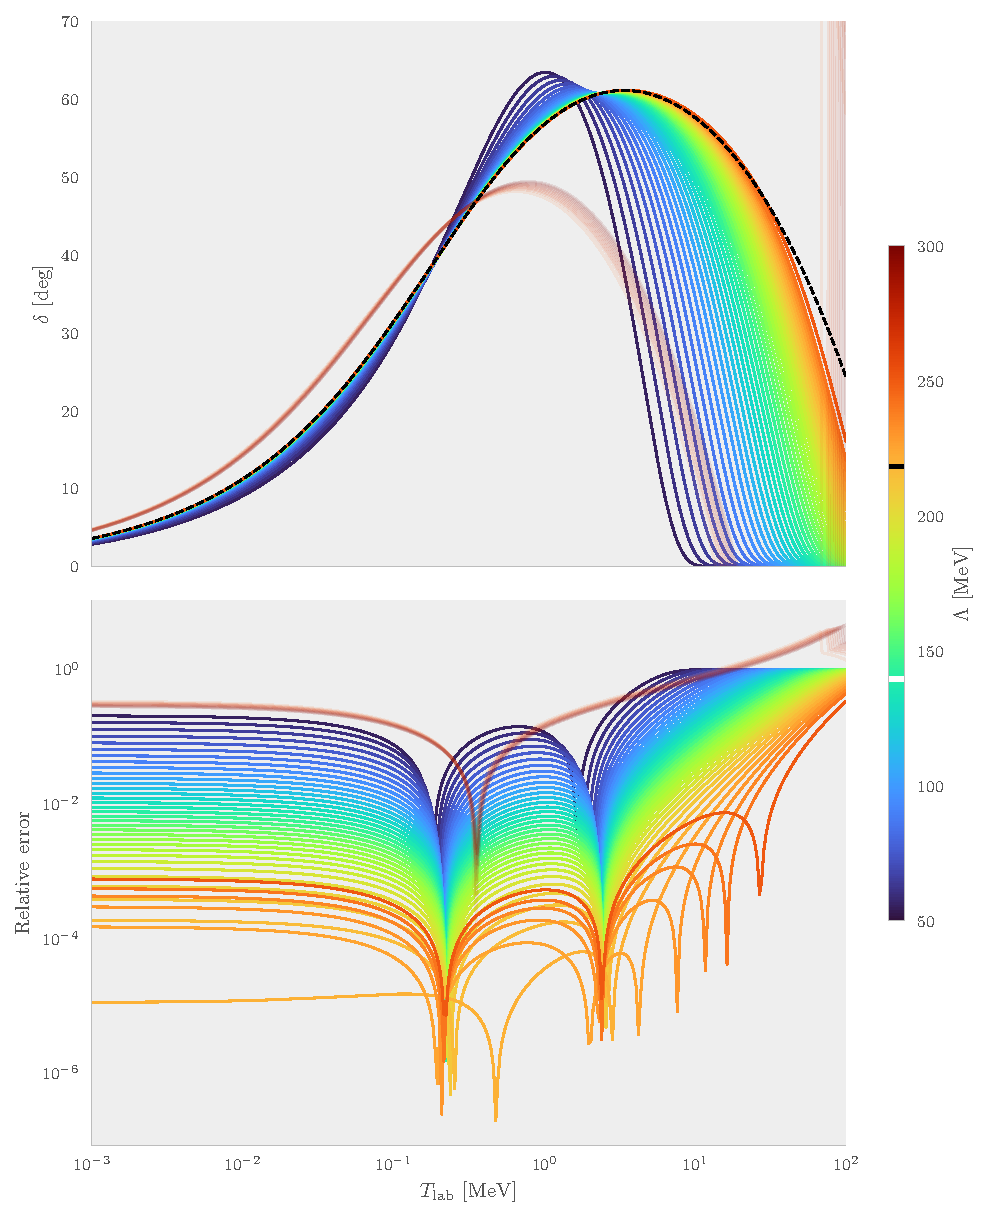
\includegraphics{Figures/lambda_LO_pion.pdf}
%   \caption{\label{fig:lambda_LO_pion_err} }
% \end{figure}


% \begin{figure}[pt]
%   \centering
%   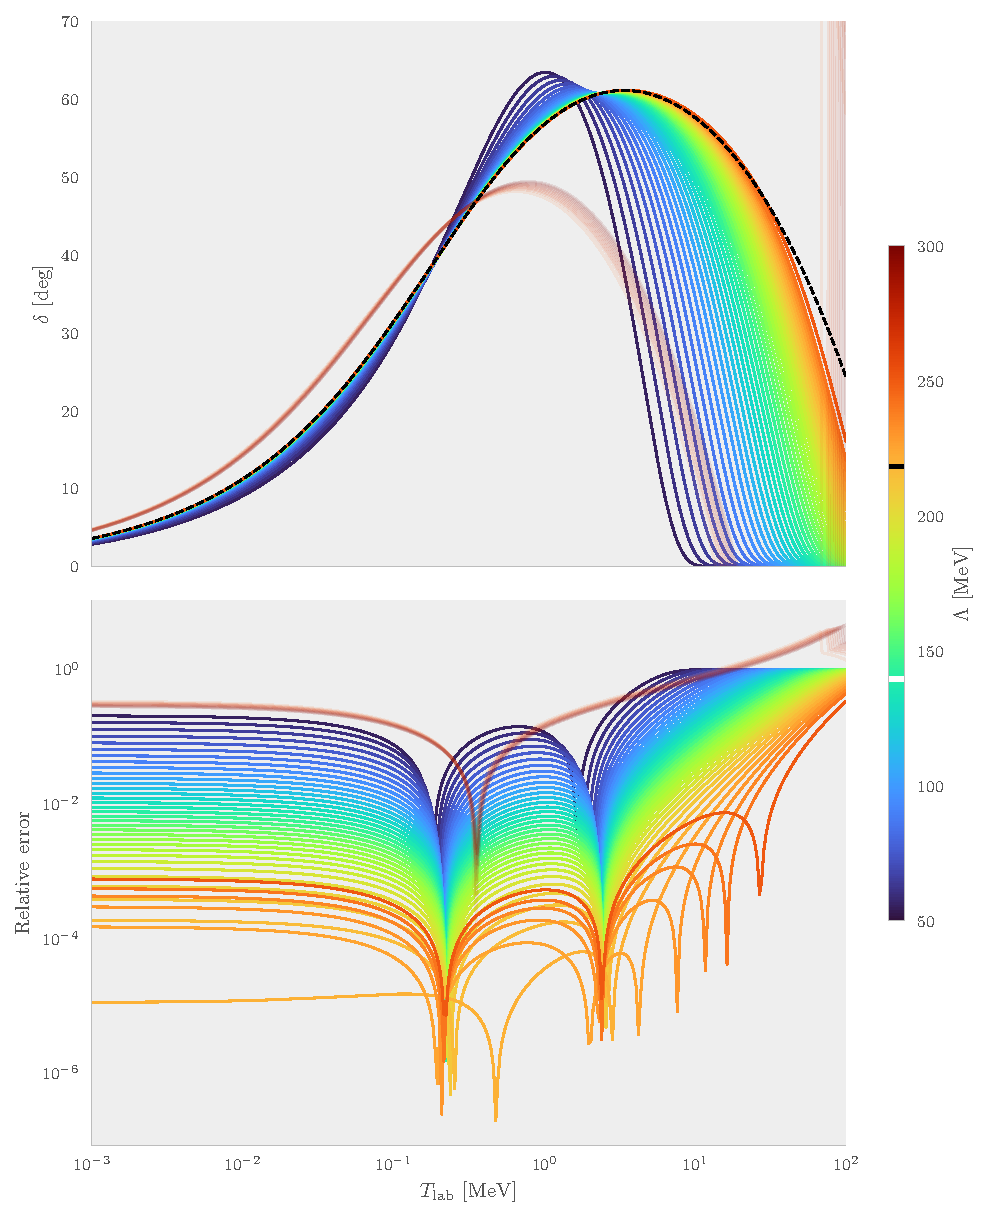
\includegraphics{Figures/lambda_LO_pion.pdf}
%   \caption{\label{fig:lambda_LO_pion} }
% \end{figure}

% \begin{figure}[pt]
%   \centering
%   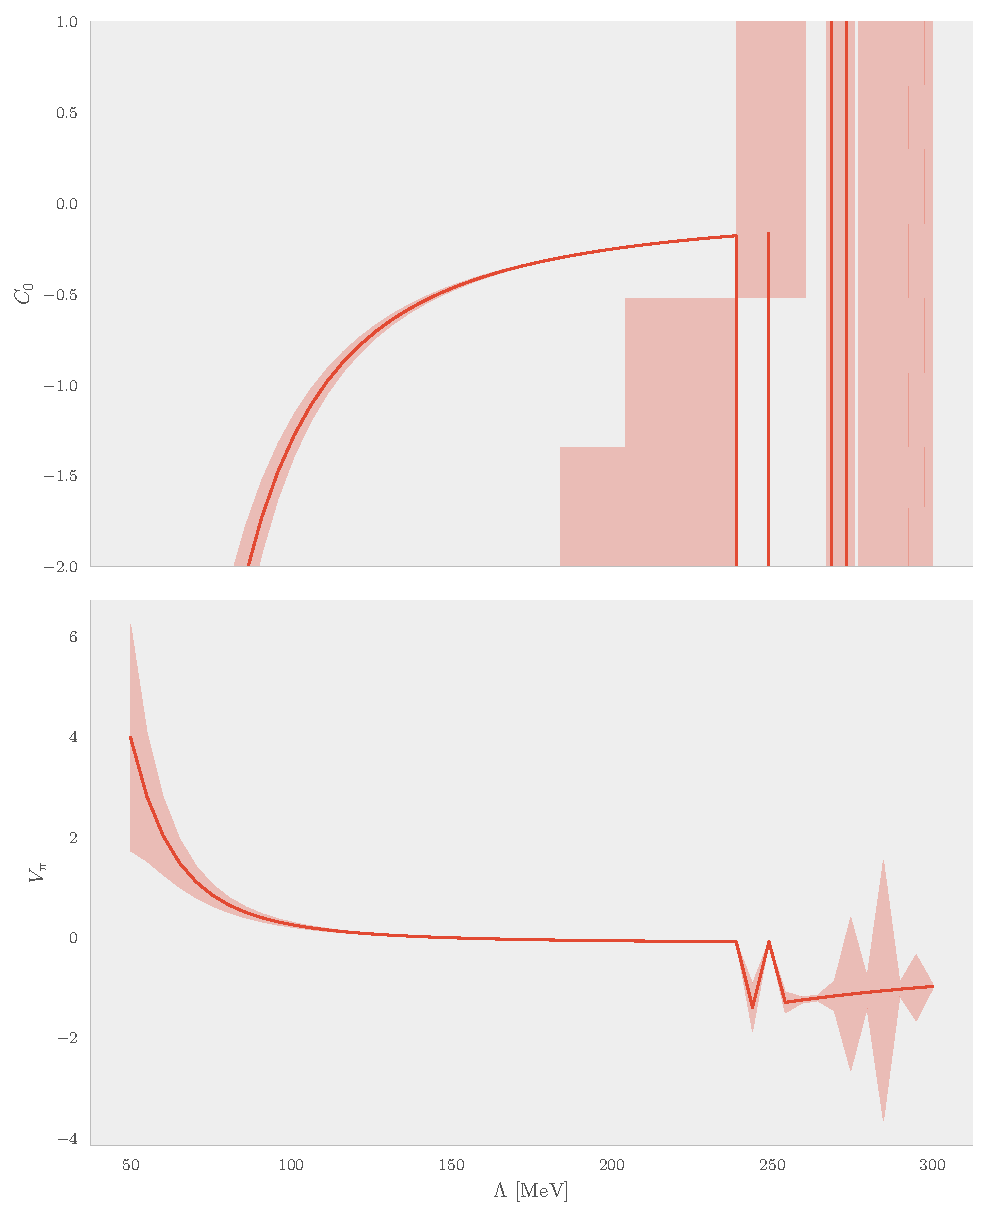
\includegraphics{Figures/lambda_coeff_LO_pion.pdf}
%   \caption{\label{fig:lambda_coeff_LO_pion} }
% \end{figure}

% \subsubsection{NLO + Pion}

% \begin{figure}[pt]
%   \centering
%   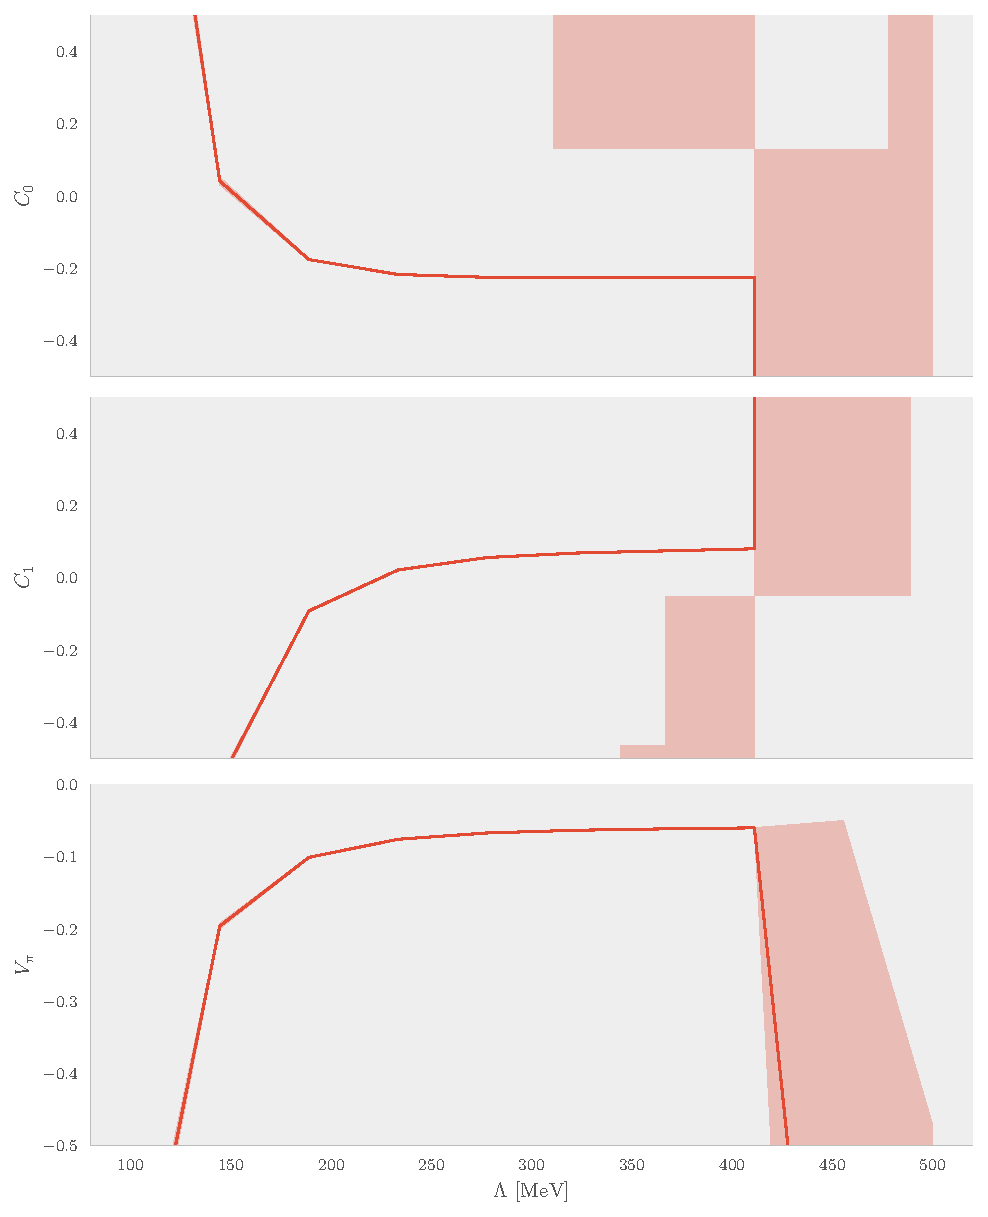
\includegraphics{Figures/lambda_coeff_NLO_pion.pdf}
%   \caption{\label{fig:lambda_NLO_pion_err} }
% \end{figure}


% \begin{figure}[pt]
%   \centering
%   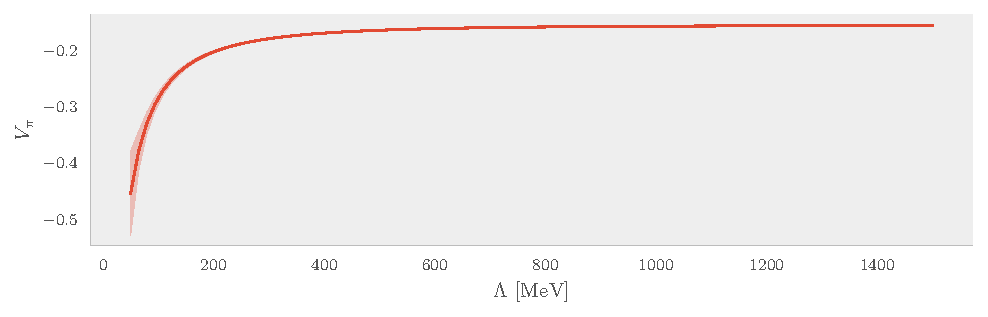
\includegraphics{Figures/lambda_NLO_pion.pdf}
%   \caption{\label{fig:lambda_NLO_pion} }
% \end{figure}

% \begin{figure}[pt]
%   \centering
%   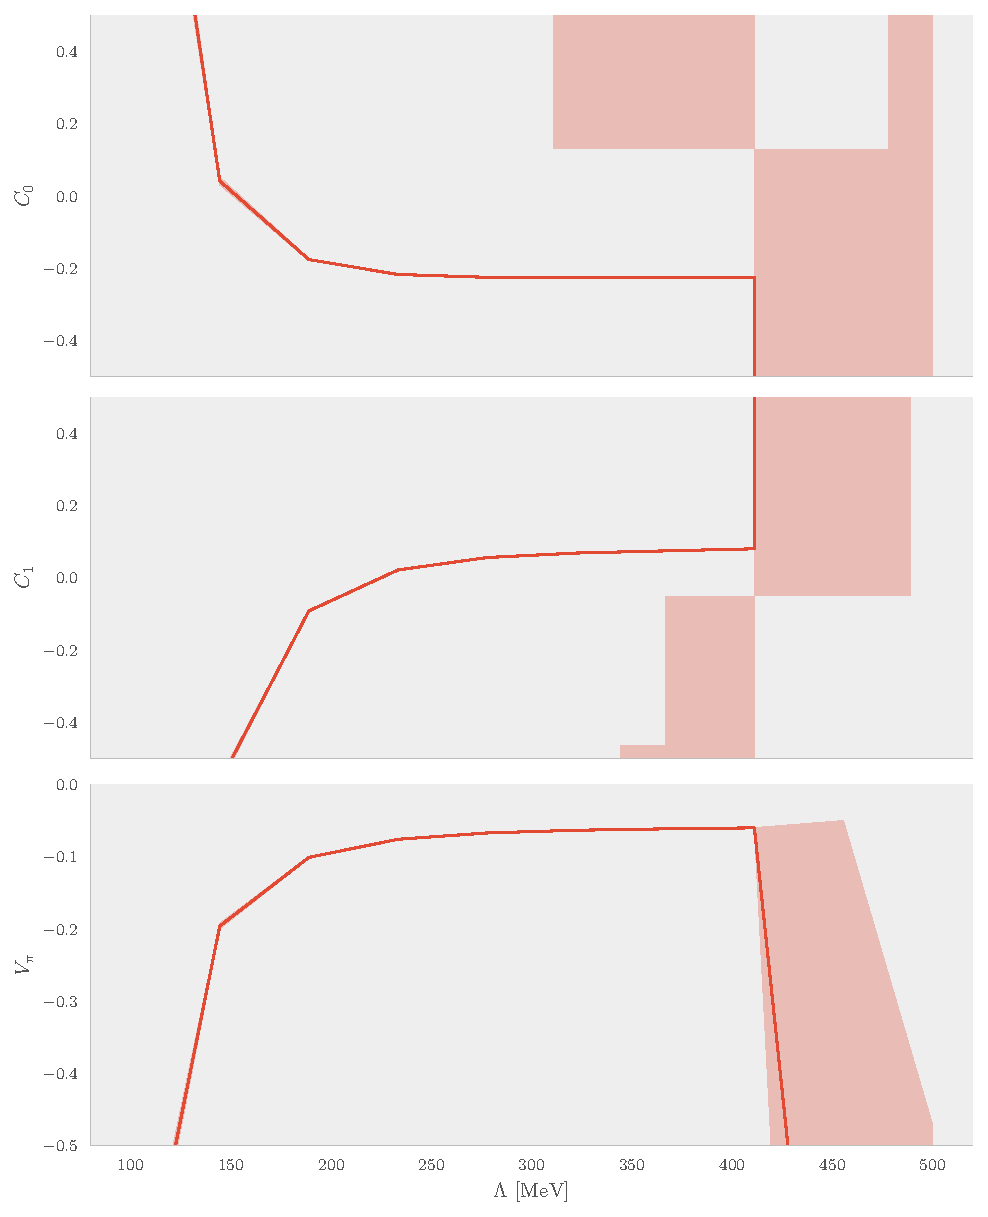
\includegraphics{Figures/lambda_coeff_NLO_pion.pdf}
%   \caption{\label{fig:lambda_coeff_NLO_pion} }
% \end{figure}

% \subsubsection{NNLO + Pion}


% \subsection{Breakdown of the K-Matrix method}
% \label{sec:breakdown-k-matrix}


% The initial coefficients were \(C_{0} = -0.5, C_{2}=-0.1\),
% \(\Lambda=\SI{0.7}{fm^{-1}}\). There were 50 points within the fit region, and
% the KMatrix method used \(30\) points.

% \begin{figure}[p]
%   \centering
%   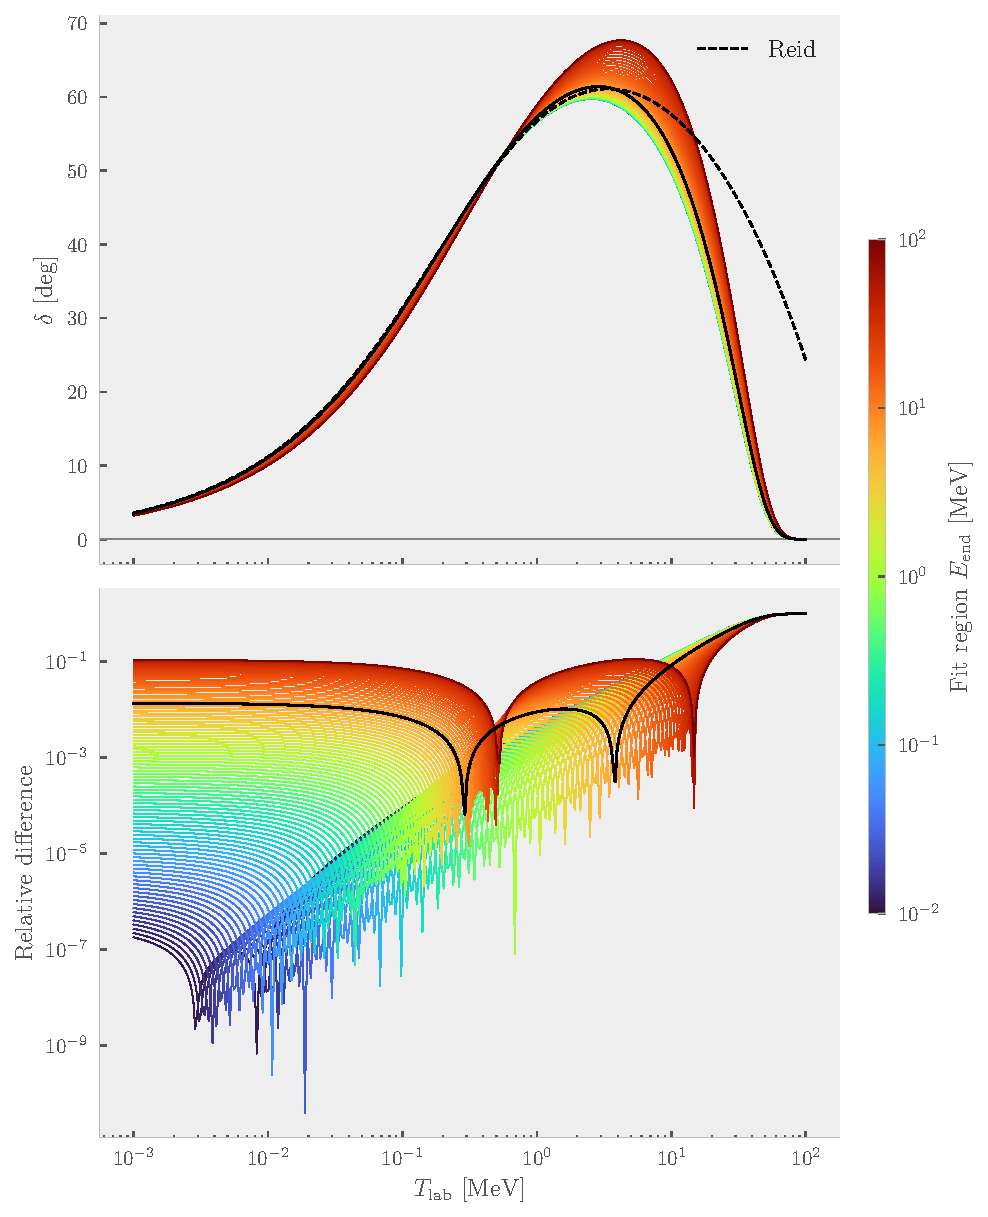
\includegraphics{Figures/NLO_region_error.pdf}
%   \caption{\label{fig:region_pointwise} Comparison of Reid and NLO with
%     different fit regions. Each curve is fit to the region \([10^{-3},
%     E_{\mathrm{end}}]\), with the optimized parameters used to compute the phase
%   shift in \([10^{-3}, 20]\), shown in the upper panel. The relative error
%   compared with Reid is shown in the lower panel. The spikes are artifacts of
%   change of sign, and should be ignored. The curves are colored by the value of
%   \(E_{\mathrm{end}}\) used in the fit. As expected the fit is better at lower
%   values when \(E_{\mathrm{end)}}\) is low, however, large \(E_{\mathrm{end}}\)
%   give drastically worse error. All of the errors converge for \(E > 10\)~MeV.}
% \end{figure}

% \begin{figure}[p]
%   \centering
%   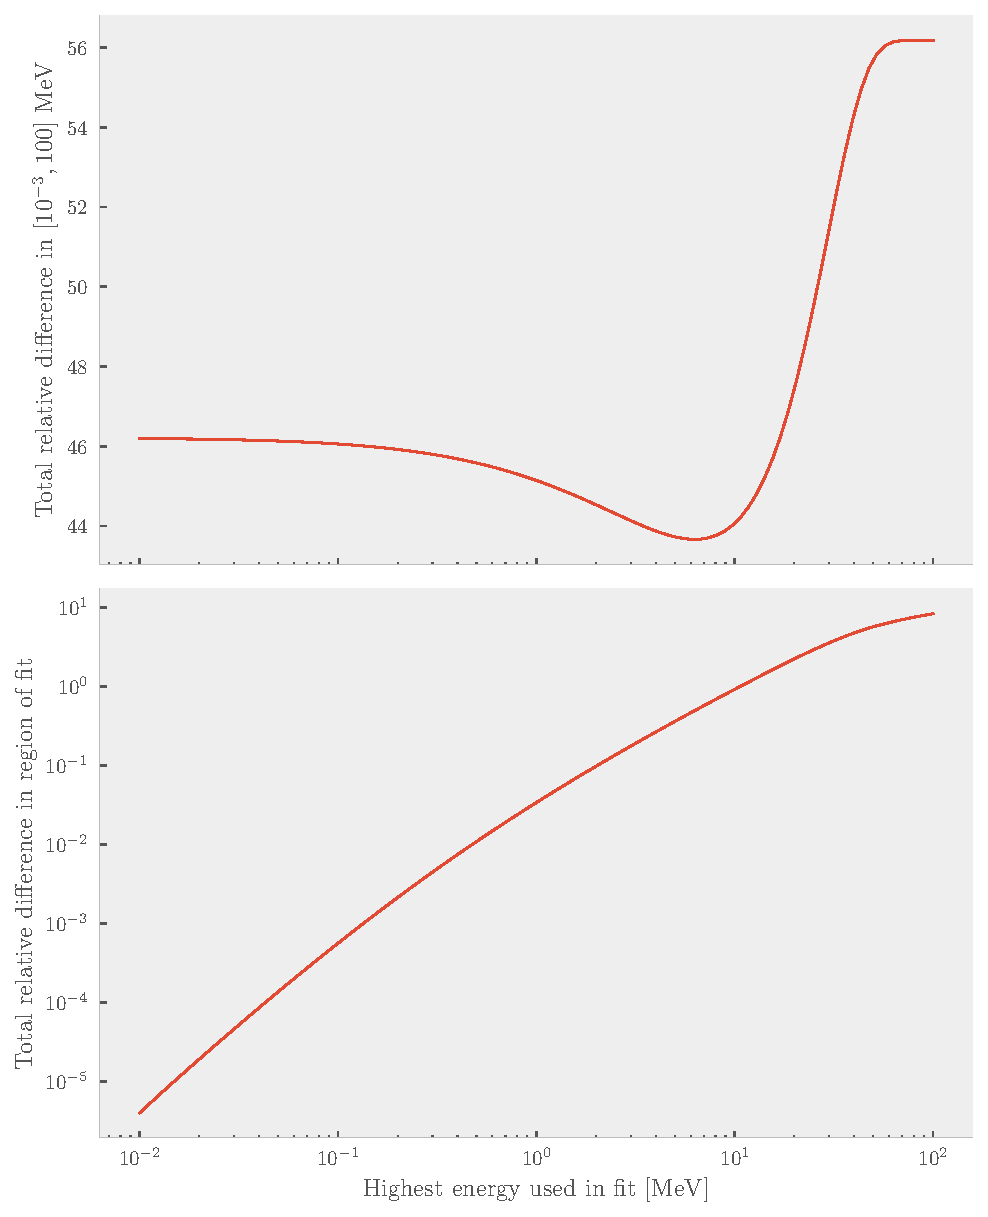
\includegraphics[]{Figures/NLO_dependence_points_error.pdf}
%   \caption{\label{fig:region_total} The time usage (top panel) and total
%     relative error (bottom panel) versus the fit region. The NLO
%     potentials are fit to the region \([\SI{1e-3}{MeV},
%     E_{\mathrm{end}}]\), with the optimized parameters used to compute the phase
%     shift in \([\SI{1e-3}{MeV}, \SI{20}{MeV}]\) and compared to the ``true'' Reid potential. The
%     relative error is summedm giving the curve in the bottom panel. For very low
%     values of \(E_{\mathrm{end}}\) the error is large. The same goes for high
%     values, perhaps unintuitively . The time usage is chaotic for \(E_{\mathrm{end}} <
%     \SI{5}{MeV}\), above which it increases rapidly to several minutes.}
% \end{figure}


% \begin{figure}[p]
%   \centering
%   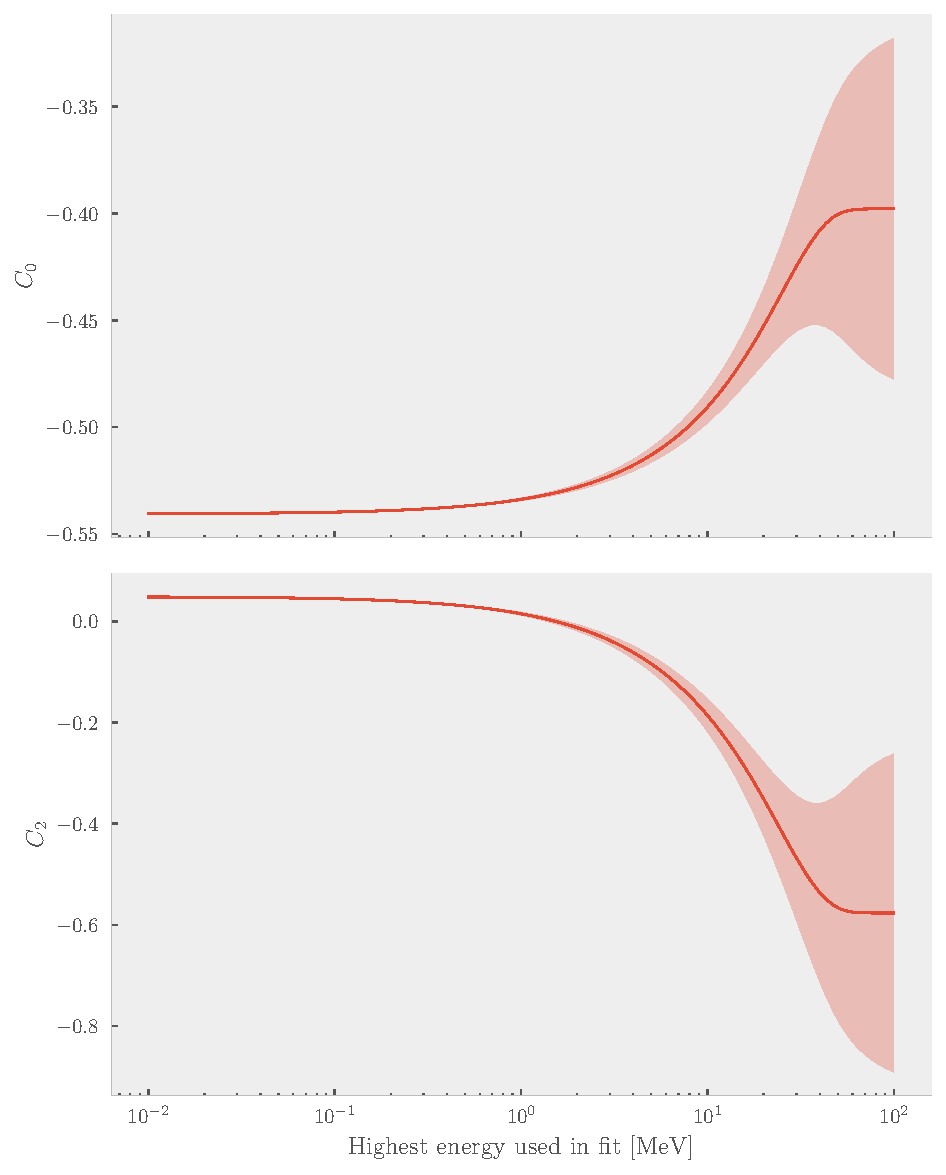
\includegraphics[]{Figures/NLO_coeff_dependence_region.pdf}
%   \caption{\label{fig:region_coeff} The dependence of the coefficients of NLO as
%   a function on \(E_{\mathrm{end}}\). There is no convergence behavior to be
%   seen in the region where the error reaches a minimum. Instead, the behavior is
% purely linear. As NLO is fit to higher energies, \(C_{0}\) increases while
% \(C_{2}\) decreases.}
% \end{figure}

% [stability]
% Coefficients must be initially given to start of the solver, and there might be
% reason for concern about the stability of the solutions. If different
% coefficients were given, would the same solution be achieved? To investigate
% this, the NLO potential was fitted fifty times with random initial coefficients in the
% interval \([-1, 1]\). For coefficients near -1, the matrix in the KMatrix method
% becomes ill conditioned, giving nonsensical results causing the solver to get
% stuck. For other initial coefficients, all solutions converge to the same
% values, agreeing within the tolerance of the optimization method. There is
% therefore no reason to suspect the solver finding local minima.


%%% Local Variables:
%%% mode: latex
%%% TeX-master: "../main"
%%% TeX-engine: xetex
%%% End:
